
\chapter{TABLESAT ATTITUDE SOFTWARE IMPLEMENTATION}
\label{chap:TableSatAttitudeDynamicsSoftware}

This chapter covers the software implementation of the attitude dynamics and control systems.  Although multiple versions of the software are created as is discussed in Chapters \ref{chap:ProgressionOfControlSystemSoftware} and \ref{chap:UNHTableSat1A}, the samples shown here are use cases of the TSatPy implementation.

\section{Implementation of Attitude Modeling}
\label{sec:ImplementationofAttitudeModeling}


\subsection{Quaternion Notation}
\label{subsec:Implementation-QuaternionNotation}

Defining a rotational quaternion using the TSatPy avoids a common issue with quaternion use where the scalar component can be placed at the leading or trailing end of the tensor depending on the author's discretion.  As is described more in Chapter \ref{chap:TSatPy}, the implementation in this thesis is done in an object oriented manner so it can handle either the scalar first or scalar last format.

\begin{singlespace}
  \begin{minted}[mathescape,linenos,numbersep=10pt,frame=lines,framesep=2mm]{python}
from TSatPy.State import Quaternion
q = Quaternion(vector=[1,2,3], scalar=4)
print(q)
q = Quaternion(scalar=0, vector=[1,2,3])
print(q)

# Prints Out
# <Quaternion [1 2 3], 4>
# <Quaternion [1 2 3], 0>
  \end{minted}
  \nocite{minted}
\end{singlespace}

\section{Rotational Quaternion}
\label{sec:Implementation-RotationalQuaternion}

The rotational quaternion is chosen as the attitude parametrization of the state vector.  As such, the two properties required to define a rotational quaternion are the Euler axis of rotation $\bs{\hat{e}}$ and the angle of rotation $\theta$.  Snippet \ref{code:make_quat_rot} demonstrates the creation of a rotational quaternion.  It also shows that proper normalization of the quaternion occurs to ensure accurate calculations.

\begin{listing}[H]
\begin{singlespace}
  \begin{minted}[mathescape,linenos,numbersep=10pt,frame=lines,framesep=2mm]{python}
from TSatPy.State import Quaternion

q = Quaternion(vector=[1,2,3], radians=4)
e, theta = q.to_rotation()

print(q)
print("Euler axis: <%g, %g, %g>" % (e[0,0], e[1,0], e[2,0]))
print("Rotation: %g radians" % theta)

# Prints Out
# <Quaternion [-0.24302 -0.48604 -0.72906], -0.416147>
# Euler axis: <-0.267261, -0.534522, -0.801784>
# Rotation: 4 radians
  \end{minted}
  \nocite{minted}
\caption{Creating a rotational quaternion}
\label{code:make_quat_rot}
\nocite{minted}
\end{singlespace}
\end{listing}

\subsection{Quaternion Multiplication}
\label{subsec:Implementation-QuaternionMultiplication}

Propagating a quaternion state accurately requires the use of the quaternion multiplication defined in \ref{eqn:QuaternionMultiplicationDerived}.  TSatPy achieves this by overriding the normal multiplication infix operator ``*''.  Snippet
\ref{code:quat_mul} demonstrates how a quaternion created from a 2 radian rotation represents the same attitude as the product of four 0.5 radian quaternions.

\begin{listing}[H]
\begin{singlespace}
  \begin{minted}[mathescape,linenos,numbersep=10pt,frame=lines,framesep=2mm]{python}
from TSatPy.State import Quaternion

a = Quaternion([1,2,3], radians=0.5)
b = Quaternion([1,2,3], radians=2)
print("a             = %s" % a)
print("a * a * a * a = %s" % (a * a * a * a))
print("b             = %s" % b)
# Prints Out
# a             = <Quaternion [-0.0661215 -0.132243 -0.198364], 0.968912>
# a * a * a * a = <Quaternion [-0.224893 -0.449785 -0.674678], 0.540302>
# b             = <Quaternion [-0.224893 -0.449785 -0.674678], 0.540302>
  \end{minted}
  \nocite{minted}
\caption{Quaternion multiplication}
\label{code:quat_mul}
\nocite{minted}
\end{singlespace}
\end{listing}

Snippet \ref{code:quat_mul_source} shows the implementation of the quaternion multiplication which reads and is used similarly to how the quaternion algebra is written.

\begin{listing}
\begin{singlespace}
  \begin{minted}[mathescape,linenos,numbersep=10pt,frame=lines,framesep=2mm]{python}
class Quaternion(object):
    def __mul__(self, q):
        v = (self.x + np.eye(3) * self.scalar) * q.vector
        v += self.vector * q.scalar
        s = self.scalar * q.scalar - (self.vector.T * q.vector)[0, 0]
        return Quaternion(v, s)
  \end{minted}
\caption{Quaternion multiplication method}
\label{code:quat_mul_source}
\nocite{minted}
\end{singlespace}
\end{listing}


\subsection{Rotating a Point with Quaternions}
\label{subsubsec:RotatingaPointwithQuaternions}

One of the main focal points of this thesis is to ensure that the tools developed in this research aide in the further development of observer-based attitude control.  To enable this goal, ``run-time'' analysis of the system is critical.  Waiting for the completion of a simulation or experimental test with TableSat IA before being able to access the information is not only an impedance to this end, but it also introduces complexity and higher ``run-time'' costs to collect and store all simulation/experimental data.  Watching representation of the system's state change as the experiment runs provides valuable insight.  In the case of an estimator, sensor voltages are converted to a measured state and the observer attempts to use it to estimate the true state of the system.  A valuable visualization is both the measured and estimated states displayed in wireframe so the effectiveness of the estimator can be readily observed.  The points in a wireframe model of TableSat can be rotated to show the estimated orientation through the use of a 3x3 rotation matrix $\bs{R}_q$ defined as
\begin{equation}
  \bs{R}_q = (q_0^2 - \bs{v}^T \bs{v}) \bs{I} + 2 \bs{v} \bs{v}^T - 2 q_0 (\bs{v} \times)
  \label{eqn:RotationMatrix}
\end{equation}

For example, for a $\pi/2$ radian rotation about $\bs{\hat{e}} = 0\bs{i}+0\bs{j}+1\bs{k}$, the rotational quaternion as defined in Equation (\ref{eqn:RotationalQuaternionDefinition}) becomes $q = 0\bs{i}+0\bs{j}-1/\sqrt{2}\bs{k}+1/\sqrt{2}$.  With Equation (\ref{eqn:RotationMatrix}), the rotational matrix becomes

\begin{equation}
  \begin{aligned}
    \bs{R_q} & = \left[ (1/\sqrt{2})^2 - (1/\sqrt{2})^2 \right] \bs{I} + 2 \begin{bmatrix} 0 & 0 & 0 \\ 0 & 0 & 0 \\ 0 & 0 & 1/\sqrt{2} \end{bmatrix} - 2 \frac{1}{\sqrt{2}} \begin{bmatrix} 0 & 1/\sqrt{2} & 0 \\ -1/\sqrt{2} & 0 & 0 \\ 0 & 0 & 0 \\ \end{bmatrix} \\
      & = \begin{bmatrix} 0 & -1 & 0 \\ 1 & 0 & 0 \\ 0 & 0 & 1 \\\end{bmatrix}
  \end{aligned}
\end{equation}

For the visualization, a point $A (2, 4, -1)$ that is in the standard orientation of body axes aligned with the global reference frame can be drawn at the current estimated location.  That is,

\begin{equation}
  A' = \bs{R_q} A = \begin{bmatrix} 0 & -1 & 0 \\ 1 & 0 & 0 \\ 0 & 0 & 1 \\\end{bmatrix} \begin{bmatrix} 2 \\ 4 \\ -1 \end{bmatrix} = \begin{bmatrix} -4 \\ 2 \\ -1 \end{bmatrix}
\end{equation}

The equivalent TSatPy implementation of the point rotation equation (Equation (\ref{eqn:RotationMatrix}))
\begin{singlespace}
  \begin{minted}[mathescape,linenos,numbersep=10pt,frame=lines,framesep=2mm]{python}
from TSatPy.State import Quaternion
import numpy as np

A = np.mat([2, 4, -1]).T
q = Quaternion([0,0,1], radians=np.pi/2)

print(q.rmatrix * A)

# Prints out
# [[-4.]
#  [ 2.]
#  [-1.]]
  \end{minted}
  \nocite{minted}
\end{singlespace}


\subsection{Quaternion-based Attitude Visualization}
\label{subsubsec:QuaternionbasedAttitudeVisualization}

% One of the largest challenges with running both simulations and live control models is having access to meaningful representations of how the system is performing.  NSS simulations are generally performed through either running of m-file scripts and analyzing logged data in a batch format after the run, or using a NSS to produce line plots of values tracked during the simulation run.


The method for calculating the new position of a point from an initial position can be extended to a collection of points that create a wireframe for the TableSat model.  Once this base wireframe is defined, the estimated attitude of the system can be visualized.  That is, if the system's estimator determines that TableSat is at an attitude of $\bs{q} = -0.38\bs{i}-0.07\bs{j}+0.91\bs{k}+0.16$, for example, this is equivalent to a 161 degree rotation about the Euler axis $\bs{\hat{e}} = 0.3844\bs{i}+0.0708\bs{j}-0.9205\bs{k}$.  Figure \ref{fig:TSatWireframe} shows the TableSat wireframe in its default configuration with its body axes aligned with the global reference frame.  The red dashed line represents the axis of rotation.

% Ideally, generating and updating a rendered model of the system at simulation time can improve the ability to attain the desired system behavior.

\begin{figure}[H]
  \centerline{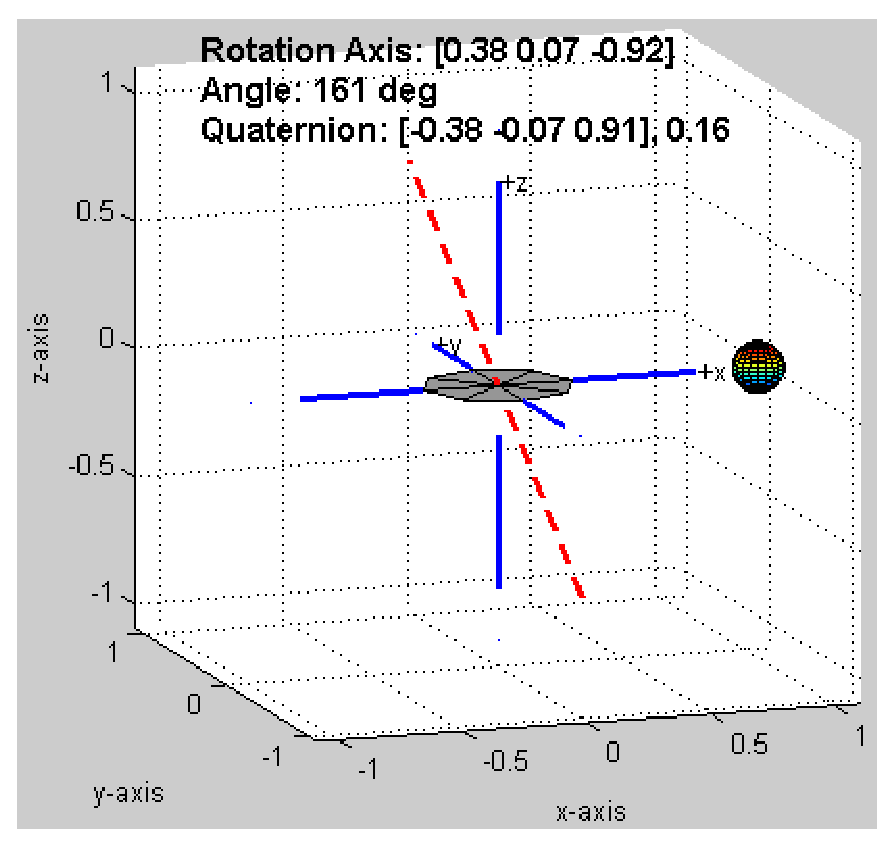
\psfig{file=figures/q_rotation_start.eps,height=3in}}
  \caption{TableSat Wireframe}
  \label{fig:TSatWireframe}
\end{figure}

Once new locations for all points in the wireframe are determined, it can be redrawn visualizing the estimated current orientation of the TableSat.  Figure \ref{fig:TSatWireframeEstimatedAttitude} shows the rotated wireframe along with the path of the body-fixed $+x$-axis traced in green.  ``Run-time'' visualizations update these representations as the simulation or experiment is occuring and shows how well the estimator runs dynamically. (discussed in greater detail in Section \ref{sec:ObjectOrientedNSSControlSystem})

\begin{figure}[H]
  \centerline{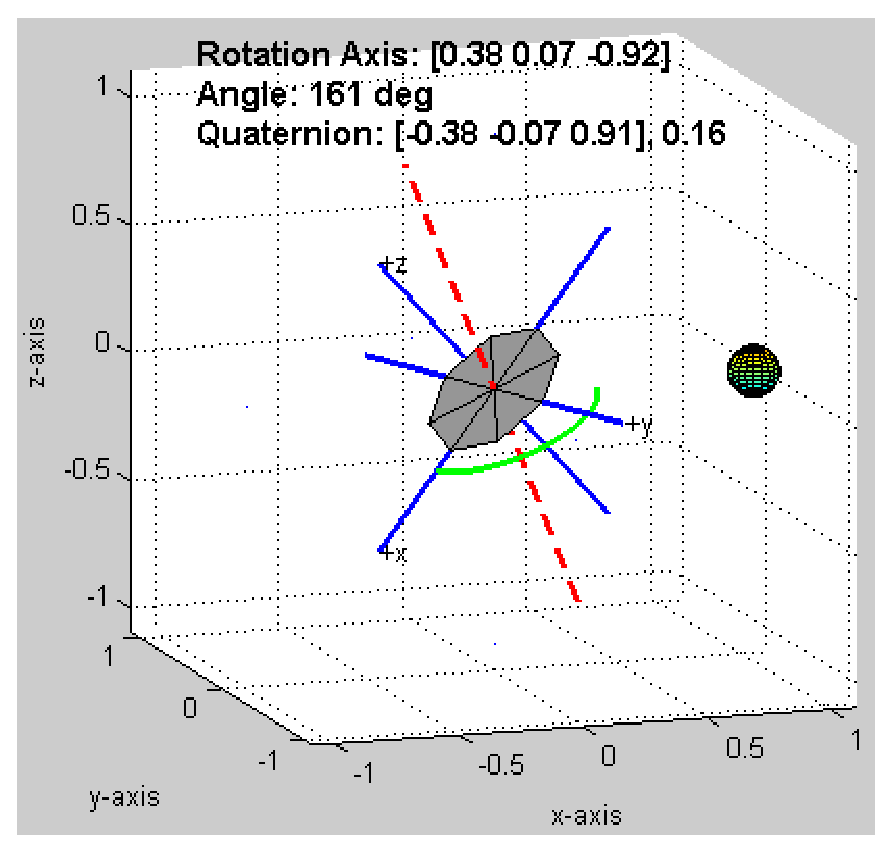
\psfig{file=figures/q_rotation_end.eps,height=3in}}
  \caption{TableSat Wireframe Estimated Attitude}
  \label{fig:TSatWireframeEstimatedAttitude}
\end{figure}


\subsection{Incremental Quaternion Rotations}
\label{subsubsec:IncrementalQuaternionRotations}

The quaternion's definition based on Euler's theorem of a rotation about a single axis simplifies the process of tracking the orientation of a spin-stabilized satellite.  NASA's MMS spacecraft has a mission spin rate of 3 rpm (~0.314 rad/sec).  A rotational quaternion, $\bs{q}_{rps}$, representing the per second rotation about the z-axis is

\begin{equation}
  \begin{aligned}
    \bs{q}_{rps} = & ( 0\bs{i} + 0\bs{j} + 1\bs{k} ) \sin \left( \frac{-0.314}{2} \right) + \cos \left( \frac{-0.314}{2} \right) \\
    = & 0\bs{i} +0\bs{j} -0.156434\bs{k} + 0.987688
  \end{aligned}
\end{equation}

In an open loop system, the best prediction of the state is to apply the quaternion rotation at each second to the previous steps state prediction, and the prediction is initialized with a known orientation.  For example, if TableSat performs a $+1/4$ turn about the z-axis each second, the best prediction at the current attitude can be obtained using just a quaternion multiplication as follows

\begin{equation}
  \begin{aligned}
    \bs{q}(t_{k+1}) = & \bs{q}_{rps} \otimes \bs{q}(t_{k}) \\
    \text{where } \bs{q}(t_0) = & 0 \bs{i} +0 \bs{j} -0.707107 \bs{k} +0.707107
  \end{aligned}
  \label{eqn:3rpmQuaternionEquation}
\end{equation}

Using the TSatPy code, Equation (\ref{eqn:3rpmQuaternionEquation}) can be implemented as

\begin{singlespace}
  \begin{minted}[mathescape,linenos,numbersep=10pt,frame=lines,framesep=2mm]{python}
from TSatPy.State import Quaternion
import time
import numpy as np

q_rps = Quaternion([0,0,1], radians=np.pi/10)
print('Quaternion spin rate (rad/sec)\n %s' % q_rps)

q_state = Quaternion([0,0,1], radians=np.pi/2)
print('Initial state of TableSat\n t=0: %s' % q_state)


print('Starting Open Loop State Tracking')
for k in range(1,11):
    time.sleep(1)
    q_state *= q_rps
    print(' t=%s: %s' % (k, q_state))

# Prints Out
# Quaternion spin rate (rad/sec)
#  <Quaternion [-0 -0 -0.156434], 0.987688>
# Initial state of TableSat
#  t=0: <Quaternion [-0 -0 -0.707107], 0.707107>
# Starting Open Loop State Tracking
#  t=1: <Quaternion [0 0 -0.809017], 0.587785>
#  t=2: <Quaternion [0 0 -0.891007], 0.45399>
#  t=3: <Quaternion [0 0 -0.951057], 0.309017>
#  t=4: <Quaternion [0 0 -0.987688], 0.156434>
#  t=5: <Quaternion [0 0 -1], 1.11022e-16>
#  t=6: <Quaternion [0 0 -0.987688], -0.156434>
#  t=7: <Quaternion [0 0 -0.951057], -0.309017>
#  t=8: <Quaternion [0 0 -0.891007], -0.45399>
#  t=9: <Quaternion [0 0 -0.809017], -0.587785>
#  t=10: <Quaternion [0 0 -0.707107], -0.707107>
  \end{minted}
  \nocite{minted}
\end{singlespace}

This method has a significant issue.  The theoretical concern is the estimate is that running in an open loop fashion without receiving correction updates.  Therefore, the myriad of additional factors in a real system would quickly invalidate the accuracy of this approach.  The implementation issue deals with the time step.  Even if TableSat spins perfectly at 3 rpm, the state is not updated exactly on each second.  A busy processor, numerical drift, and execution time would prevent the desired fixed step size of 1 sec.  In some of the earlier implementations of the base station controller (discussed in Chapter \ref{chap:ProgressionOfControlSystemSoftware}), dropped UDP messages cause the control loop to execute on an inconsistent interval and prevent accurate state estimates.  (Handling of the variability in time steps is discussed in Section \ref{sec:SatelliteDynamics})


\subsection{Quaternion Decomposition}
\label{subsec:TSatPyQuaternionDecomposition}

The need for a quaternion decomposition is noted in Section \ref{subsec:QuaternionDecompositionForNutationControl} of the controls chapter and the method for performing the decomposition is derived in \ref{subsec:QuaternionDecomposition}.  Snippet \ref{code:sample_quaternion_decomposition} shows a this functionality as built in the TSatPy software through the decomposition of a quaternion representing a 1 radian rotation about the Euler axis $[0 \ 0.1 \ 1]^T$

\begin{listing}[H]
\begin{singlespace}
  \begin{minted}[mathescape,linenos,numbersep=10pt,frame=lines,framesep=2mm]{python}
from TSatPy.State import State, Quaternion, BodyRate

print("State Error")
x_e = State(
    Quaternion([0,0.1,1],radians=1),
    BodyRate([0,-0.01,0.2]))
print("x_e: %s" % (x_e))

print("Decomposed Quaternion")
q_r, q_n = x_e.q.decompose()
print("q_r: %s" % q_r)
print("q_n: %s" % q_n)

print("Nutation Only State Error")
x_e.q = q_n
print("x_e: %s" % (x_e))

# Prints Out
# State Error
# x_e: <Quaternion [-0 -0.0477046 -0.477046], 0.877583>,
#      <BodyRate [0 -0.01 0.2]>
# Decomposed Quaternion
# q_r: <Quaternion [0 0 -0.47759], 0.878583>
# q_n: <Quaternion [-0.0227833 -0.0419125 -0], -0.998861>
# Nutation Only State Error
# x_e: <Quaternion [-0.0227833 -0.0419125 -0], -0.998861>,
#      <BodyRate [0 -0.01 0.2]>
  \end{minted}
\caption{Quaternion decomposition}
\label{code:sample_quaternion_decomposition}
\nocite{minted}
\end{singlespace}
\end{listing}




\section{Satellite Dynamics}
\label{sec:SatelliteDynamics}

One of the goals in creating an accurate dynamic model is to predict the state of the system given the last know state, the elapsed time since the last known state, and any inputs to the system.  The initial scope of predicting the satellite's state is restricting it to a state propagation problem where only last state and elapsed time are considered.  (Estimation techniques in Section \ref{chap:Estimators} describes how a propagated state can be adjusted using the measured state.)

\subsection{System Clock}
\label{subsec:SystemClock}

As mentioned previously, the chance of having perfectly timed updates is highly unlikely.  Small variations in the time step size results in errors.  A state update running every 1.0001 seconds instead of every second would accumulate over a six degree error after tracking TableSat's state for an hour.  A linearized model is also affected because the expected time step size is incorporated as part of the discretization processes.

The preset fixed time step is also not very fault tolerant.  When controlling the state of a stable, slow moving system the state, the tracking rate can be decreased to conserve system resources.  In this circumstance a missed or series of missed updates due to faults can cause the predicted state to lag by be several time steps.  A variable step sized based solution can improve the robustness against these errors.

The ability to decrease the simulation speed to enable more detailed inspection of the initial transient behavior and to increase simulation speed to enable inspection of long term system stability hold significant benefits for this research.  The TSatPy system is designed to address the previous two issues as the system needs to be able to smoothly transition between variations in step sizes in a single experimental test such that

\begin{equation}
  t_k = \sum\limits_{i=0}^{k-1} r_i (\tau_{i+1} - \tau_i)\\
  \label{eqn:SystemTime}
\end{equation}
where $\tau$ represents true time and $t_k$ denotes the time at step $k$

The system clock defined in Equation (\ref{eqn:SystemTime}) initializes at zero and increases accordingly for varying step sizes.  TSatPy implements this concept through the Metronome class as shown in Snippet \ref{code:metronome}.  An instance of this class serves as the reference frame for all rate calculations.  During the simulation, the clock is able to adjust speed according to varying set speed.

\begin{listing}[H]
\begin{singlespace}
  \begin{minted}[mathescape,linenos,numbersep=10pt,frame=lines,framesep=2mm]{python}
from TSatPy.Clock import Metronome
import time

c = Metronome()
print("Start Time: system=%s, real=%s" % (c, time.time()))
time.sleep(2)
print("Lock step:  system=%s, real=%s" % (c, time.time()))
c.set_speed(0.1)
time.sleep(30)
print("Slow-mo:    system=%s, real=%s" % (c, time.time()))
c.set_speed(100)
time.sleep(4)
print("FFW:        system=%s, real=%s" % (c, time.time()))

# Prints Out
# Start Time: system=7.86781e-06s, real=1396147884.5
# Lock step:  system=2.00162s, real=1396147886.5
# Slow-mo:    system=5.00364s, real=1396147916.52
# FFW:        system=405.292s, real=1396147920.52
  \end{minted}
\caption{Metronome}
\label{code:metronome}
\nocite{minted}
\end{singlespace}
\end{listing}


\subsection{Body Rate and Quaternion Propagation}
\label{subsec:BodyRateQuaternionPropagation}

Predicting the body rates $\omega_x, \omega_y,$ and $\omega_z$ for TableSat requires knowledge of the body dynamics, the last calculated body rate, time elapsed since last update, and any applied moments.  Equation (\ref{eqn:DiscreteEulerMomentEquations}) is used to propagate the body rate taking into account variable step sizes.

\begin{singlespace}
  \begin{minted}[mathescape,linenos,numbersep=10pt,frame=lines,framesep=2mm]{python}
from TSatPy.Clock import Metronome
from TSatPy import State
import time

clock = Metronome()

M = [0, 0, 0.5]
w = State.BodyRate([0, 0, 0])
eme = State.EulerMomentEquations(
    [[10, 0, 0], [0, 10, 0], [0, 0, 10]], w, clock)

for k in range(5):
    w = eme.propagate(M)
    print(w)
    time.sleep(1)

# Prints Out
# <BodyRate [0 0 0]>
# <BodyRate [0 0 0.0500562]>
# <BodyRate [0 0 0.10012]>
# <BodyRate [0 0 0.150189]>
# <BodyRate [0 0 0.200252]>
  \end{minted}
\nocite{minted}
\end{singlespace}

The quaternion propagation operates in the same way as the body rate propagation, and Equation (\ref{eqn:DiscreteQuaternionPropagation}) is implemented in the QuaternionDynamics (Chapter \ref{chap:tsatpy_source}).  Snippet \ref{code:quaternion_prop_clock} describes a basic quaternion propagation where the TableSat model is tracking a 0.1 rad/sec rotation about the $+z$ axis.  The system clock initially tracks in real time (e.g. a second of real elapsed time roughly equates to the equivalent system time change).  After each update the angle increases by about 0.1 rad.  After a four second transient response period, the speed of the system clock is increased by a factor of five (line 19).  After that each step simulates a 0.5 rad increase from when the clock speed changed.

\begin{listing}[H]
\begin{singlespace}
  \begin{minted}[mathescape,linenos,numbersep=10pt,frame=lines,framesep=2mm]{python}

from TSatPy.Clock import Metronome
from TSatPy import State
import time

c = Metronome()
print("Setting spin rate of 0.1 rad/sec about +z")
w = State.BodyRate([0, 0, 0.1])
q_ic = State.Identity()

qd = State.QuaternionDynamics(q_ic, c)

for _ in range(4):
    time.sleep(1)
    e, theta = qd.propagate(w).to_rotation()
    print(" Rotation Angle: %s" % theta)

print("Initial transient response inspection complete.")
print("Speed up 5x for steady state response.")
c.set_speed(5)

for _ in range(4):
    time.sleep(1)
    e, theta = qd.propagate(w).to_rotation()
    print(" Rotation Angle: %s" % theta)

# Prints Out
# Setting spin rate of 0.1 rad/sec about +z
#  Rotation Angle: 0.0
#  Rotation Angle: 0.100147199631
#  Rotation Angle: 0.203001904488
#  Rotation Angle: 0.303643703461
# Initial transient response inspection complete.
# Speed up 5x for steady state response.
#  Rotation Angle: 0.804805707932
#  Rotation Angle: 1.30787069798
#  Rotation Angle: 1.81127579212
#  Rotation Angle: 2.3147197485
  \end{minted}
\caption{Quaternion propagation with varying clock speed}
\label{code:quaternion_prop_clock}
\nocite{minted}
\end{singlespace}
\end{listing}

In this study, quaternion and body rate propagation techniques will be incorporated into the TableSat IA observer-based control system.

\section{Messages Between TableSat and the Base Station}

\subsection{Message Protocol}
\label{subsec:UDPTCP}

Communication between the controller and the experimental TableSat is negotiated over a User Datagram Protocol (UDP) socket.  Both the controller and TableSat read and write over port 9877.  UDP is used for a stateless connection more generally used for pushing data over a large number of connections.  The other common communication protocol is Transmission Control Protocol (TCP) where a session is established between server and client and successful transferral of data is acknowledged by the recipient.

Advantages and disadvantages exist between the TCP and UDP protocols and became a critical factor in influencing the design of TableSat IA base station controller. Section \ref{sec:NSSModel} goes into further detail in how this difference in protocols cropped up early in the development of the base station controller where the combination of a Numerical Simulation Software (like MATLAB Simulink or Octave) with a UDP communication protocol produced a very fragile system.

A UDP message transmission is done in a ``fire and forget'' fashion.  The message header can generally include the originating hosts ip address and port so that the server knows where to send the response.  The session-less nature of UDP means that the originating server sends the message, but does not receive confirmation that the message transmitted successfully as with TCP where ever interaction is followed up with an acknowledgment from the other host.

The advantage to using UDP for the UNH TableSat 1 is that the satellite side code could be largely based off of Melissa Vess' work on her TableSat thesis where the control loop was implemented on-board, and the UDP connection was used to infrequently poll for data or modify sensor calibration values.  The UDP connection has the slight advantage of being able to transmit and receive packets without needing to wait for acknowledgments.  This could save a small fraction of time, but on modern hardware and with the small bandwidth usage this advantage is negligible.

Disadvantages to a UDP implementing the control interface through UDP include the possibility of packet loss where the sender submits a packet, but it gets corrupted or dropped.  Since UDP is a stateless connection, the sender doesn't wait for an acknowledgment which in this case would not come. This issue is handled by the communications module.  If the control loop rate on both updating the actuator voltages and polling sensor data is fast enough, a dropped packet would not matter much since a new updated set of values would be soon to follow.  Issues could be caused if the completion of a code loop was dependent on a packet coming in.  If dropped, the control loop could block until the next packet is received.  This was one issue encountered in the project version [sec:ControlLoopinSimulink].


\subsection{Message Definitions}
\label{subsec:MessageDefinitions}


The packet structure used for this project is the same as used by Melissa Vess \cite{vessthesis}. Each UDP packet is comprised of a packet header and data payload.  The packet header format remains constant for all messages containing five octets of data.

\begin{table}[H]
  \centering
  \begin{tabular}{| l | l |}
    \hline
    Header Octet & Description \\ \hline
    h1 & Message Number (0 to 255) \\ \hline
    h2 & Flags (0 - 255) \\ \hline
    h3 & Message Size (0 - 255) \\ \hline
    h4 & Message Size (0 - 255) \\ \hline
    h5 & 0 \\ \hline
  \end{tabular}
  \caption{UDP message headers}
  \label{tbl:UDPMessageHeaders}
\end{table}

The first octet (h1) contains the message number that matches to a predefined list of messages known by both the sender and recipient.  This is used to specify how the data in the payload is to be used.

The second octet (h2) is reserved for flags.  For some messages, flags can be set for additional data.  These are not used in the final implementation of NASA MMS TableSat IA.

The third (h3) and fourth (h4) header octets define the size of the data's payload, so when reading data in from a buffer, the header can inform the recipient how many bytes need to get read in from the buffer in order to get to the end of the packet.  For payloads less than 256 bytes only the fourth header byte is needed.  For payloads larger than 255 bytes the following formula is used to specify the message size headers.

\begin{subequations}
  \begin{align}
    h4 &= mod(size, 256) \\
    h3 &= floor(size / 256)
  \end{align}
  \label{eqn:UDPSizeHeader}
\end{subequations}

The only meta data provided along with the payload beyond the data's size is an 8 bit message number.  Both UNH TableSat IA and the control station have identical message list definitions.

\begin{table}[H]
  \centering
  \begin{tabular}{|l|l|l|l|}
    \hline
    Message Id & Payload Size & Data Type & Message Description \\ \hline
    2 & 1 octet & unsigned int & Set run mode \\ \hline
    4 & 1 octet & unsigned int & Set run mode \\ \hline
    18 & 4 x (8 octets) & float & Set fan voltages \\ \hline
    19 & 1 octet & unsigned int & Set log record mode \\ \hline
    20 & 1 octet & unsigned int & Request sensor reading \\ \hline
    22 & 1 octet & unsigned int & End of sensor log \\ \hline
    23 & 8 octets & float & Request sensor log data \\ \hline
    33 & 8 octets & float & Set log sample rate \\ \hline
    63 & 15 x (8 octets) & float & Sensor readings \\ \hline
    64 & 16 x (8 octets) & float & Sensor log entry \\ \hline
    65 & 8 octets & float & Sensor log size \\ \hline
    104 & 1 octet & unsigned int & Ack run mode \\ \hline
    118 & 1 octet & unsigned int & Ack fan volt \\ \hline
    119 & 1 octet & unsigned int & Ack sensor log run mode \\ \hline
    133 & 1 octet & unsigned int & Ack log sample rate \\ \hline
  \end{tabular}
  \caption{TableSat message definitions}
  \label{tbl:UDPMessageDefinitions}
\end{table}


\section{Calculating Nutation From Three-Axis Magnetometer}

The following example shows a sample calculation of nutation based on a single set of coarse sun sensor and TAM voltage measurements.

The base station submits a request for sensor data (message id \#20) to TableSat which responds with a packet containing the sensor output voltages (message id \#63) with a payload containing 15 floats (timestamp, 6 photodiodes, 4 accelerometrs, gyroscope, and 3 three-axis magnetometer).

\subsection{Calculate Yaw From Coarse Sun Sensor}

Using sample CSS output voltages from the photodiodes (0.37247, 0.30899, 1.18370, 2.40020, 1.80500, and 0.44052), the TSatPy python package (whose development is detailed in Chapter \ref{chap:TSatPy}) uses Equation (\ref{eqn:CSSResultantForce}) to convert the sensor voltages into a meaningful state as shown in Snippet \ref{code:css_to_yaw}.

\begin{listing}[H]
\begin{singlespace}
  \begin{minted}[mathescape,
               linenos,
               numbersep=10pt,
               frame=lines,
               framesep=2mm]{python}
import TSatPy
import numpy as np

css_v = [0.37247, 0.30899, 1.18370, 2.40020, 1.80500, 0.44052]

pda = TSatPy.Sensor.PhotoDiodeArray()
pda.update_state(css_v)
vector, radians = pda.x.q.to_rotation()

print "A %g radian (%d degree) rotation about <%g, %g, %g>" % (
    radians, radians / np.pi * 180,
    vector[0,0], vector[1,0], vector[2,0])

# Prints out
# A 3.34585 radian (191 degree) rotation about <-0, -0, -1>
  \end{minted}
\caption{Converting CSS voltage outputs to a Yaw measurement}
\label{code:css_to_yaw}
\nocite{minted}
\end{singlespace}
\end{listing}

\subsection{Calculate TAM Nutation Reference Data}
\label{subsec:CalculateTAMNutationReferenceData}

Figure \ref{fig:TAMNutationVoltages} shows that while the TAM readings vary enough to be noticeable for large nutations, the signal contain a significant level of noise.  In order to use the TAM to quantify nutation for the observer-based controller, the data in Table \ref{tbl:TAMCalibration} is reduced to five data points for a yaw angle of 191 degrees.  When updating the estimator, TAM sensor values can be compared to the five reference nutation points of level, $+x$ down, $+y$ down, $-x$ down, and $-y$ down.

\begin{table}[H]
  \centering
  \begin{tabular}{c|c|c|c}
    \hline
    Yaw   & Steady & $+X \ 14^o$ & $+Y \ 14^o$ \\ \hline
    (deg) & TAM (V) & TAM (V) & TAM (V) \\ \hline
    0 & $(S_{x0},S_{y0},S_{z0})$ & $(+X_{x0},+X_{y0},+X_{z0})$ & $(+Y_{x0},+Y_{y0},+Y_{z0})$\\
    1 & $(S_{x1},S_{y1},S_{z1})$ & $(+X_{x1},+X_{y1},+X_{z1})$ & $(+Y_{x1},+Y_{y1},+Y_{z1})$\\
    2 & $(S_{x2},S_{y2},S_{z2})$ & $(+X_{x2},+X_{y2},+X_{z2})$ & $(+Y_{x2},+Y_{y2},+Y_{z2})$\\
    ... & & &  \\ \hline
    \hline
    Yaw   & $-X \ 14^o$ & $-Y \ 14^o$ \\ \hline
    (deg) & TAM (V) & TAM (V) \\ \hline
    0 & $(-X_{x0},-X_{y0},-X_{z0})$ & $(-Y_{x0},-Y_{y0},-Y_{z0})$\\
    1 & $(-X_{x1},-X_{y1},-X_{z1})$ & $(-Y_{x1},-Y_{y1},-Y_{z1})$\\
    2 & $(-X_{x2},-X_{y2},-X_{z2})$ & $(-Y_{x2},-Y_{y2},-Y_{z2})$\\
    ... & & &  \\ \hline
  \end{tabular}
  \caption{TAM calibration reference table structure}
  \label{tbl:TAMCalibration}
\end{table}

The method chosen for creating the five reference points starts with collecting approximately 2400 data points with corresponding TAM and coarse sun sensor voltage readings.  The voltages for each nutation setting are grouped into 1 degree increments.  Multiple rotations create some overlap in measurements.  The final reference value for each degree is calculated through a weighted average of a specified smoothing window.

Figure \ref{fig:TAMNutationReference} shows the result of the nutation reference values for 5, 15 and 25 degree smoothing windows.  At $\pm 15$ degrees, an adequate level of noise is filtered without causing over smoothing.  At this level, each of the 191 degree reference values are a weighted average of about 200 of the original calibration points.

\begin{figure}[H]
  \begin{subfigure}[h!]{0.8\textwidth}
    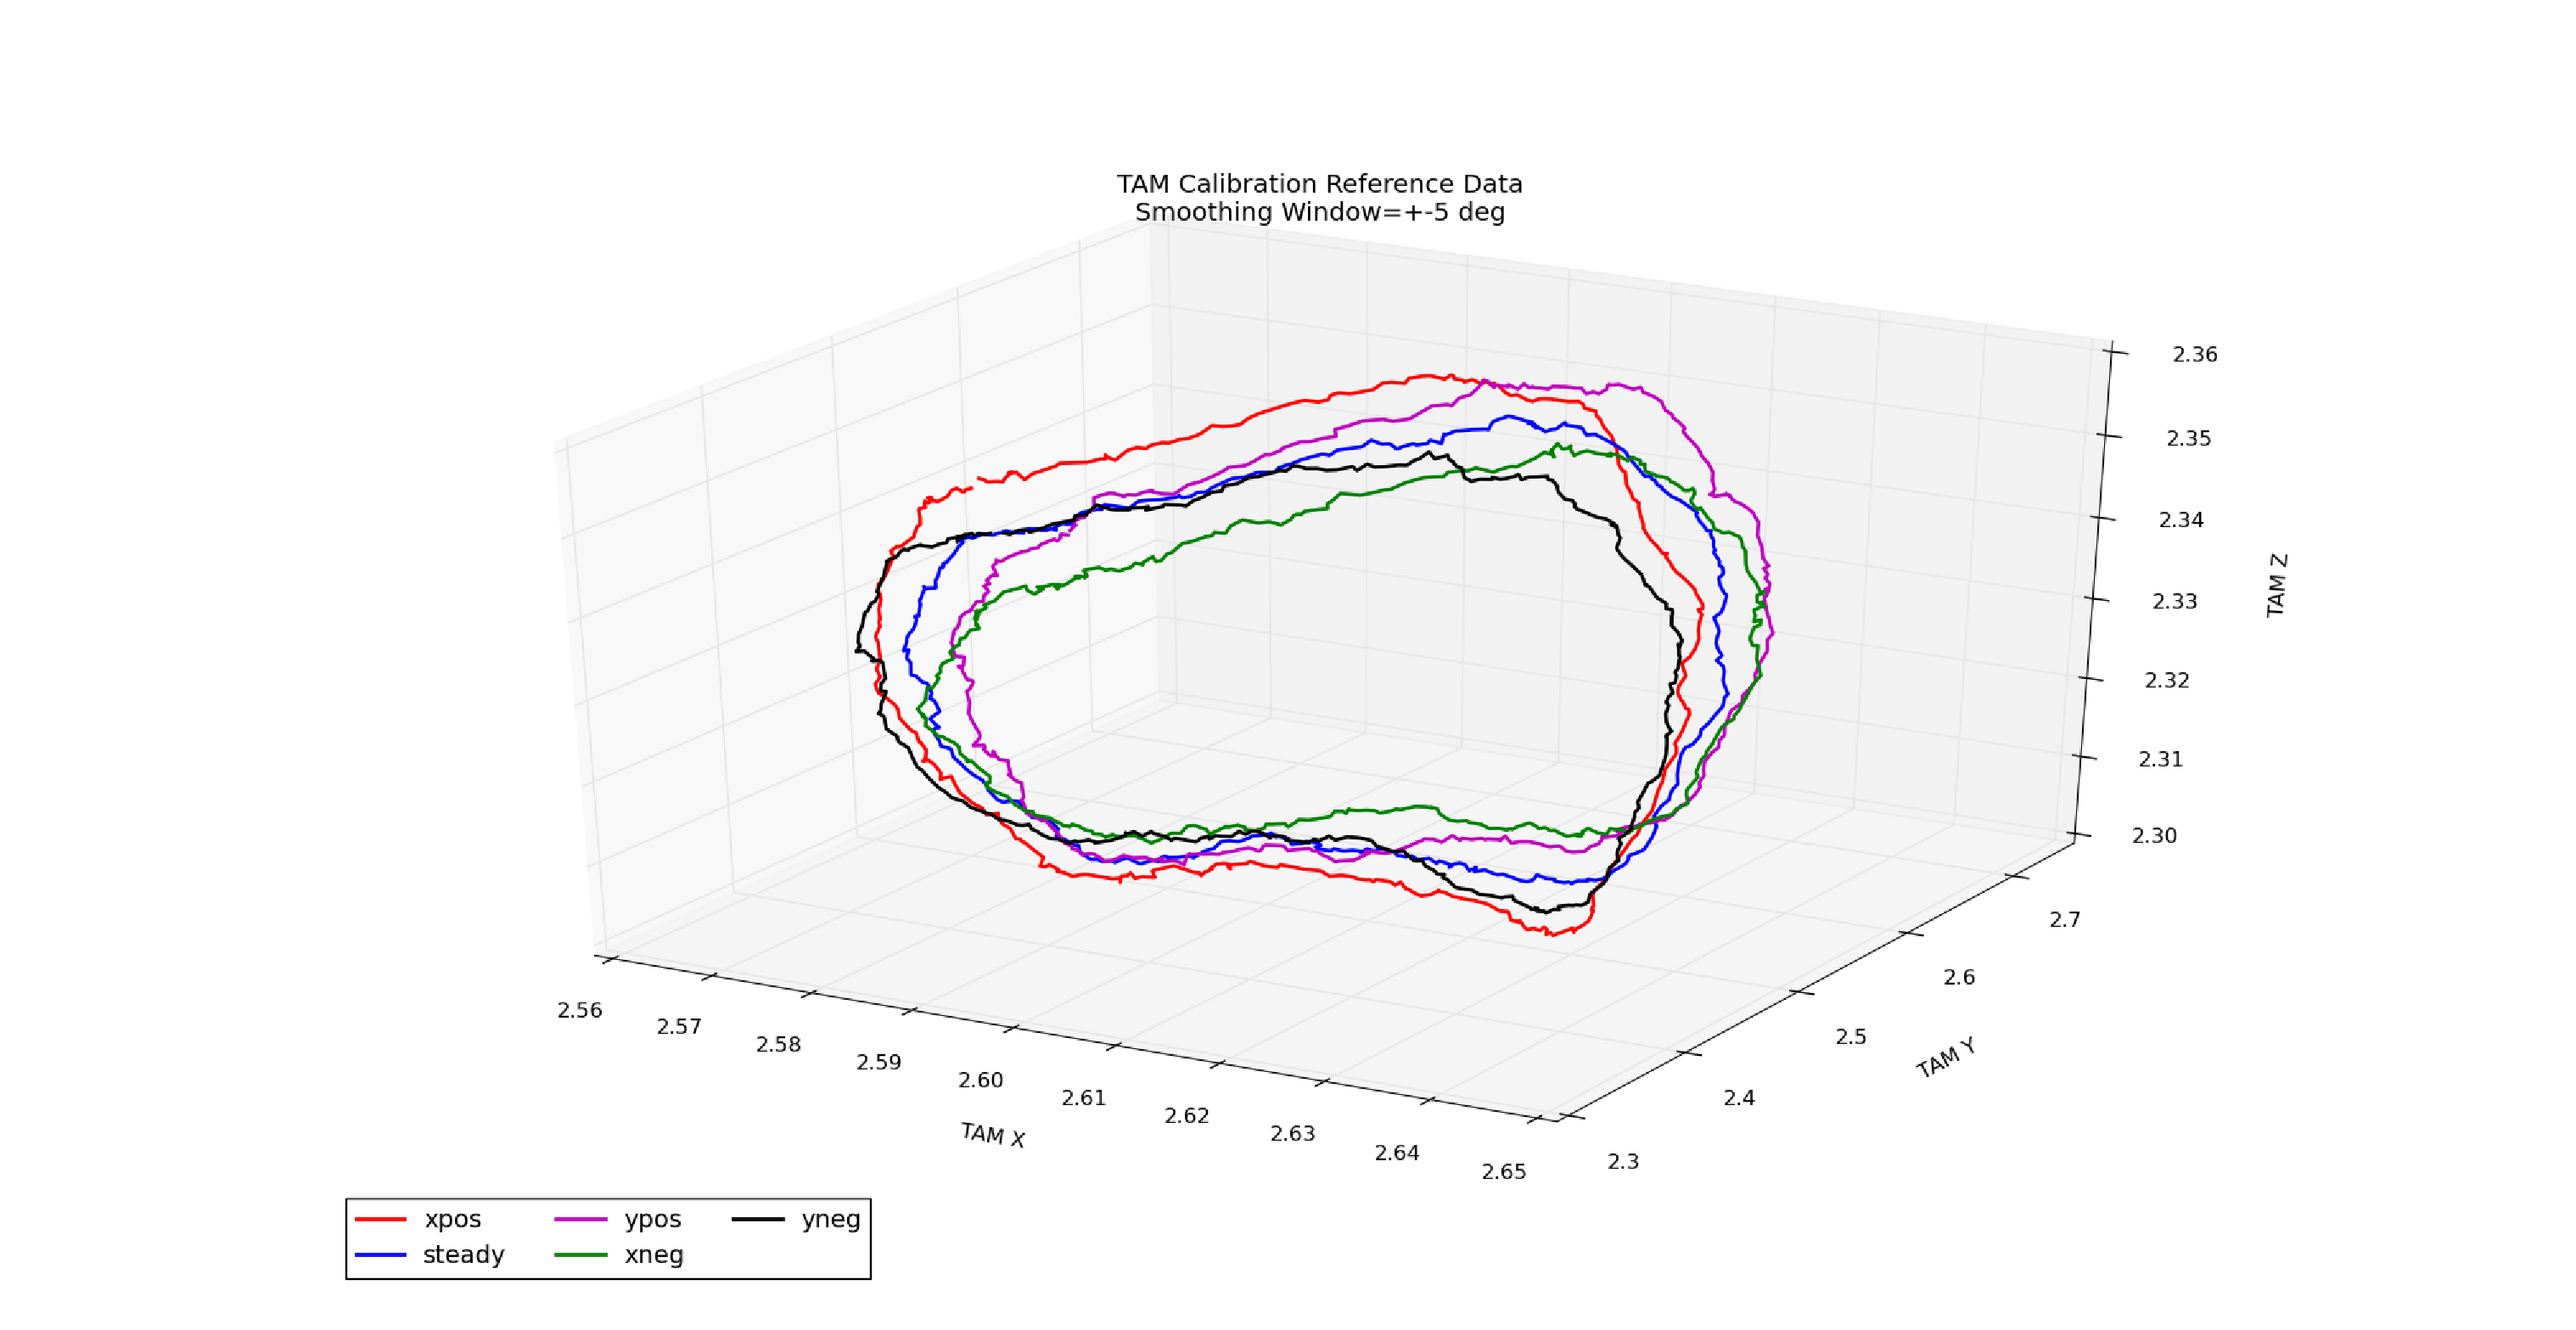
\includegraphics[width=\textwidth]{figures/tam_calibration_ref_5deg_smoothing.eps}
    \caption{$\pm 5^o$ smoothing}
    \label{fig:TAM5degCalibration}
  \end{subfigure}

  \begin{subfigure}[h!]{0.8\textwidth}
    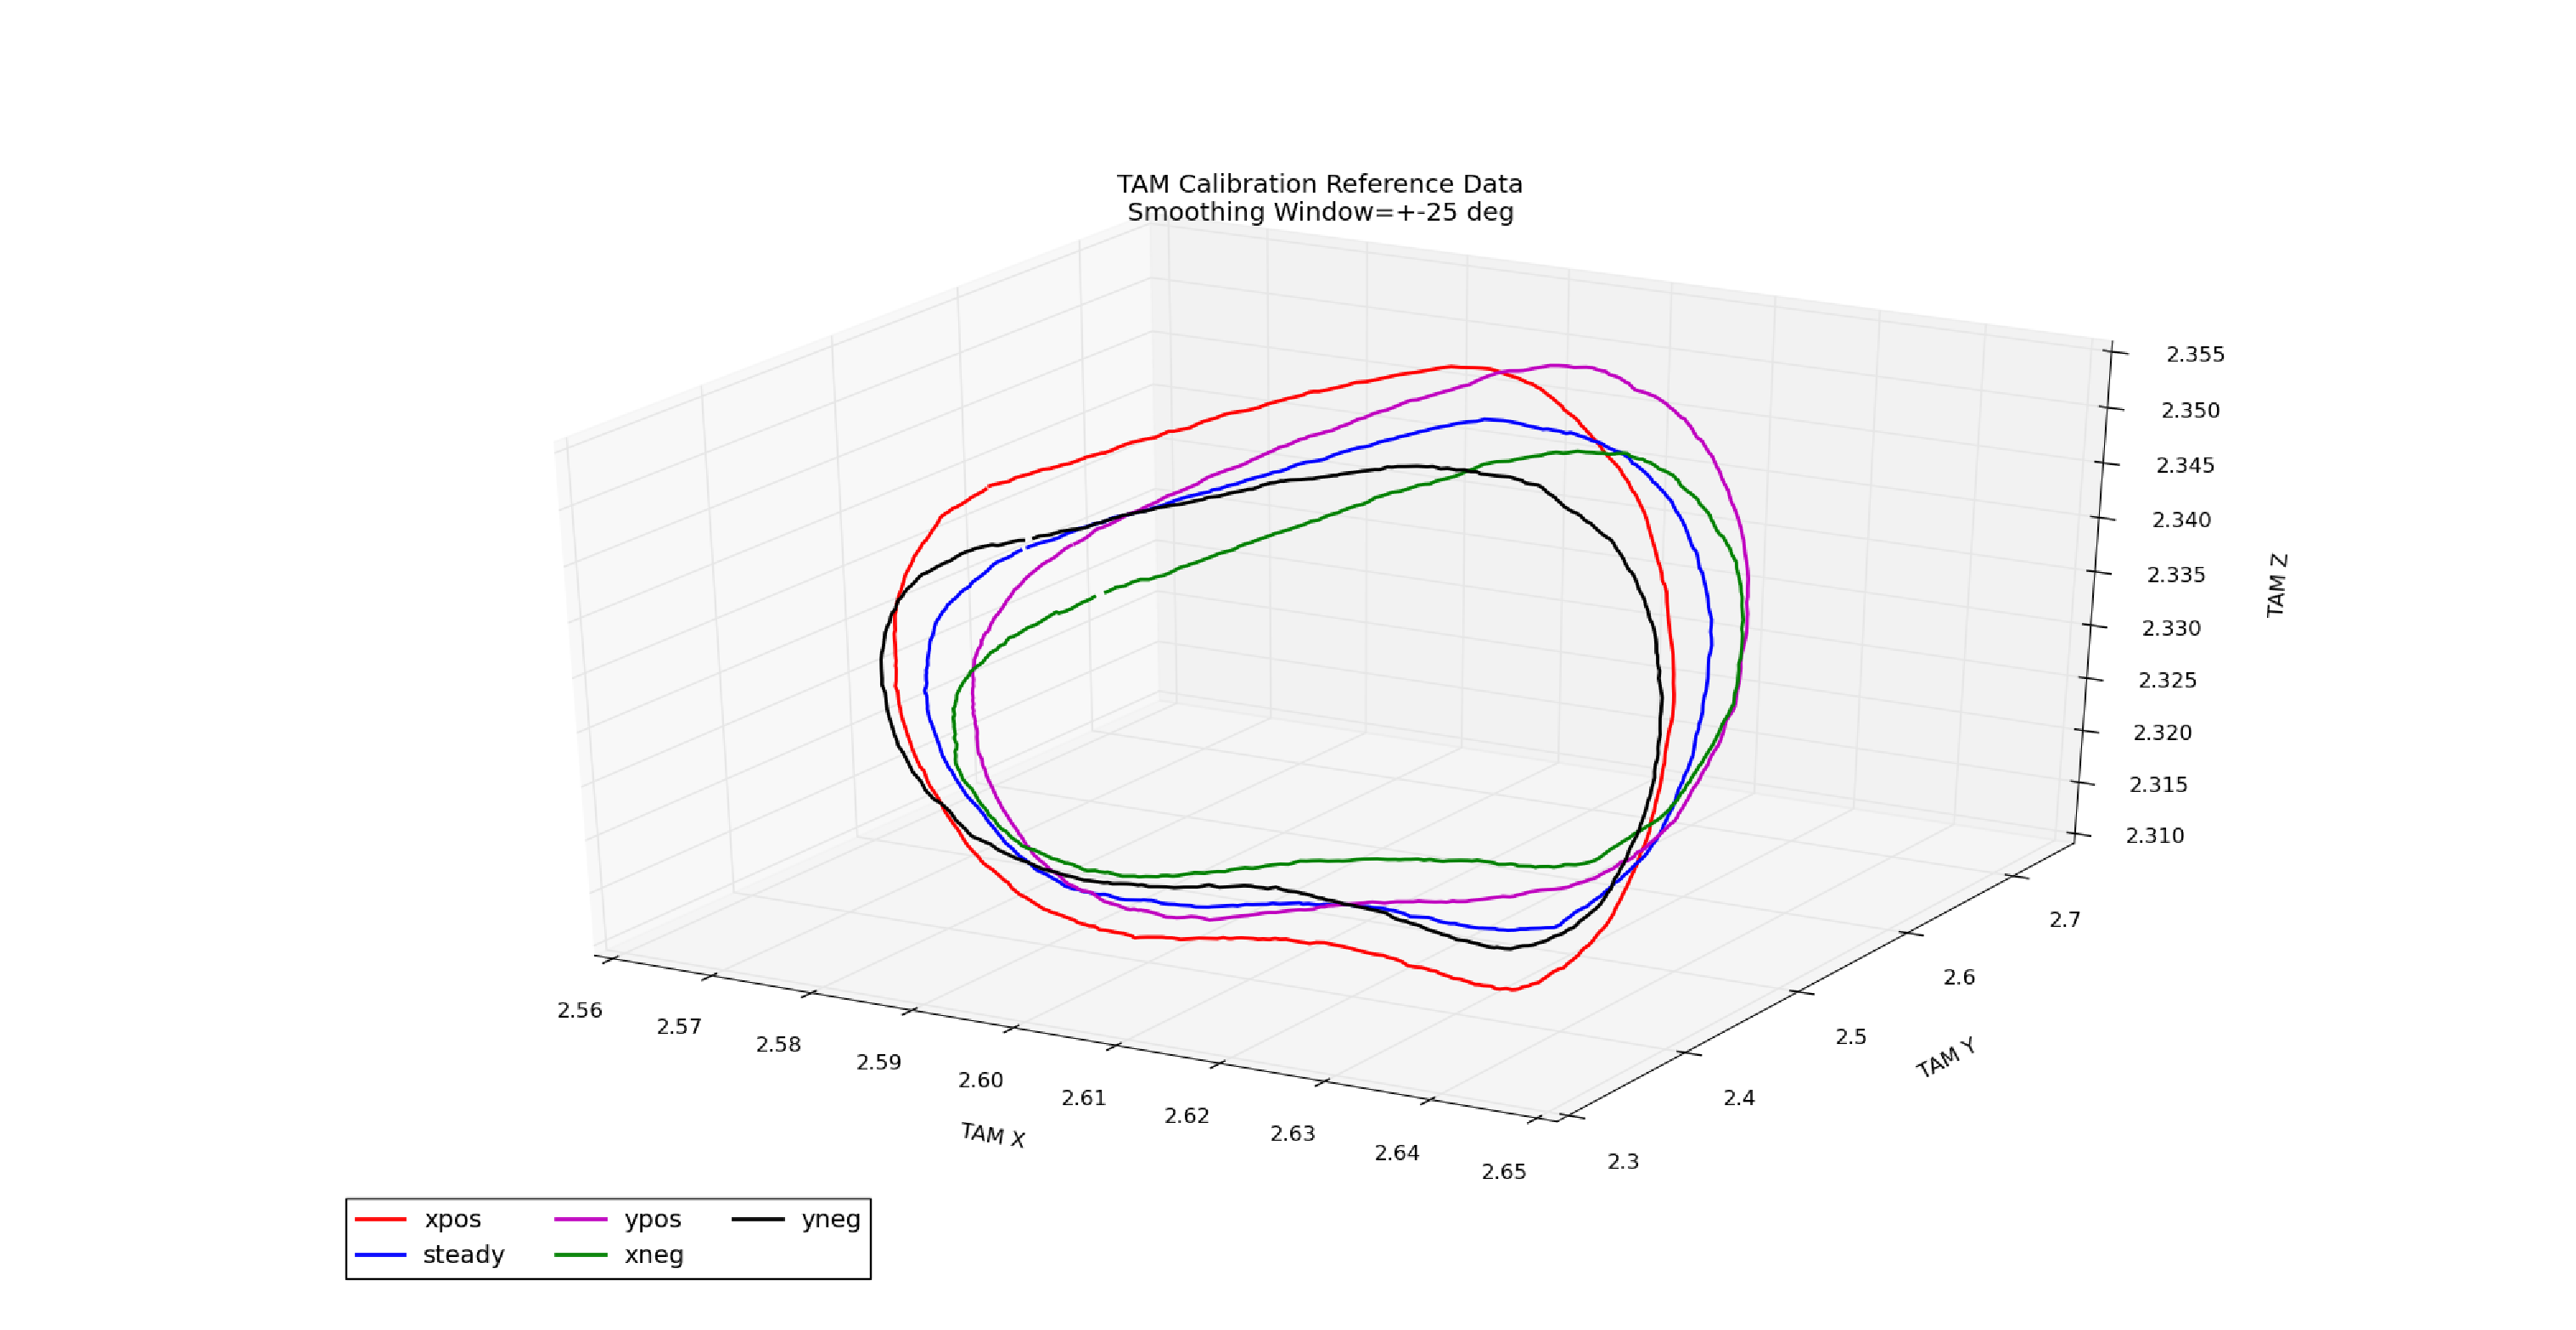
\includegraphics[width=\textwidth]{figures/tam_calibration_ref_25deg_smoothing.eps}
    \caption{$\pm 25^o$ smoothing}
    \label{fig:TAM25degCalibration}
  \end{subfigure}

  \begin{subfigure}[h!]{0.8\textwidth}
    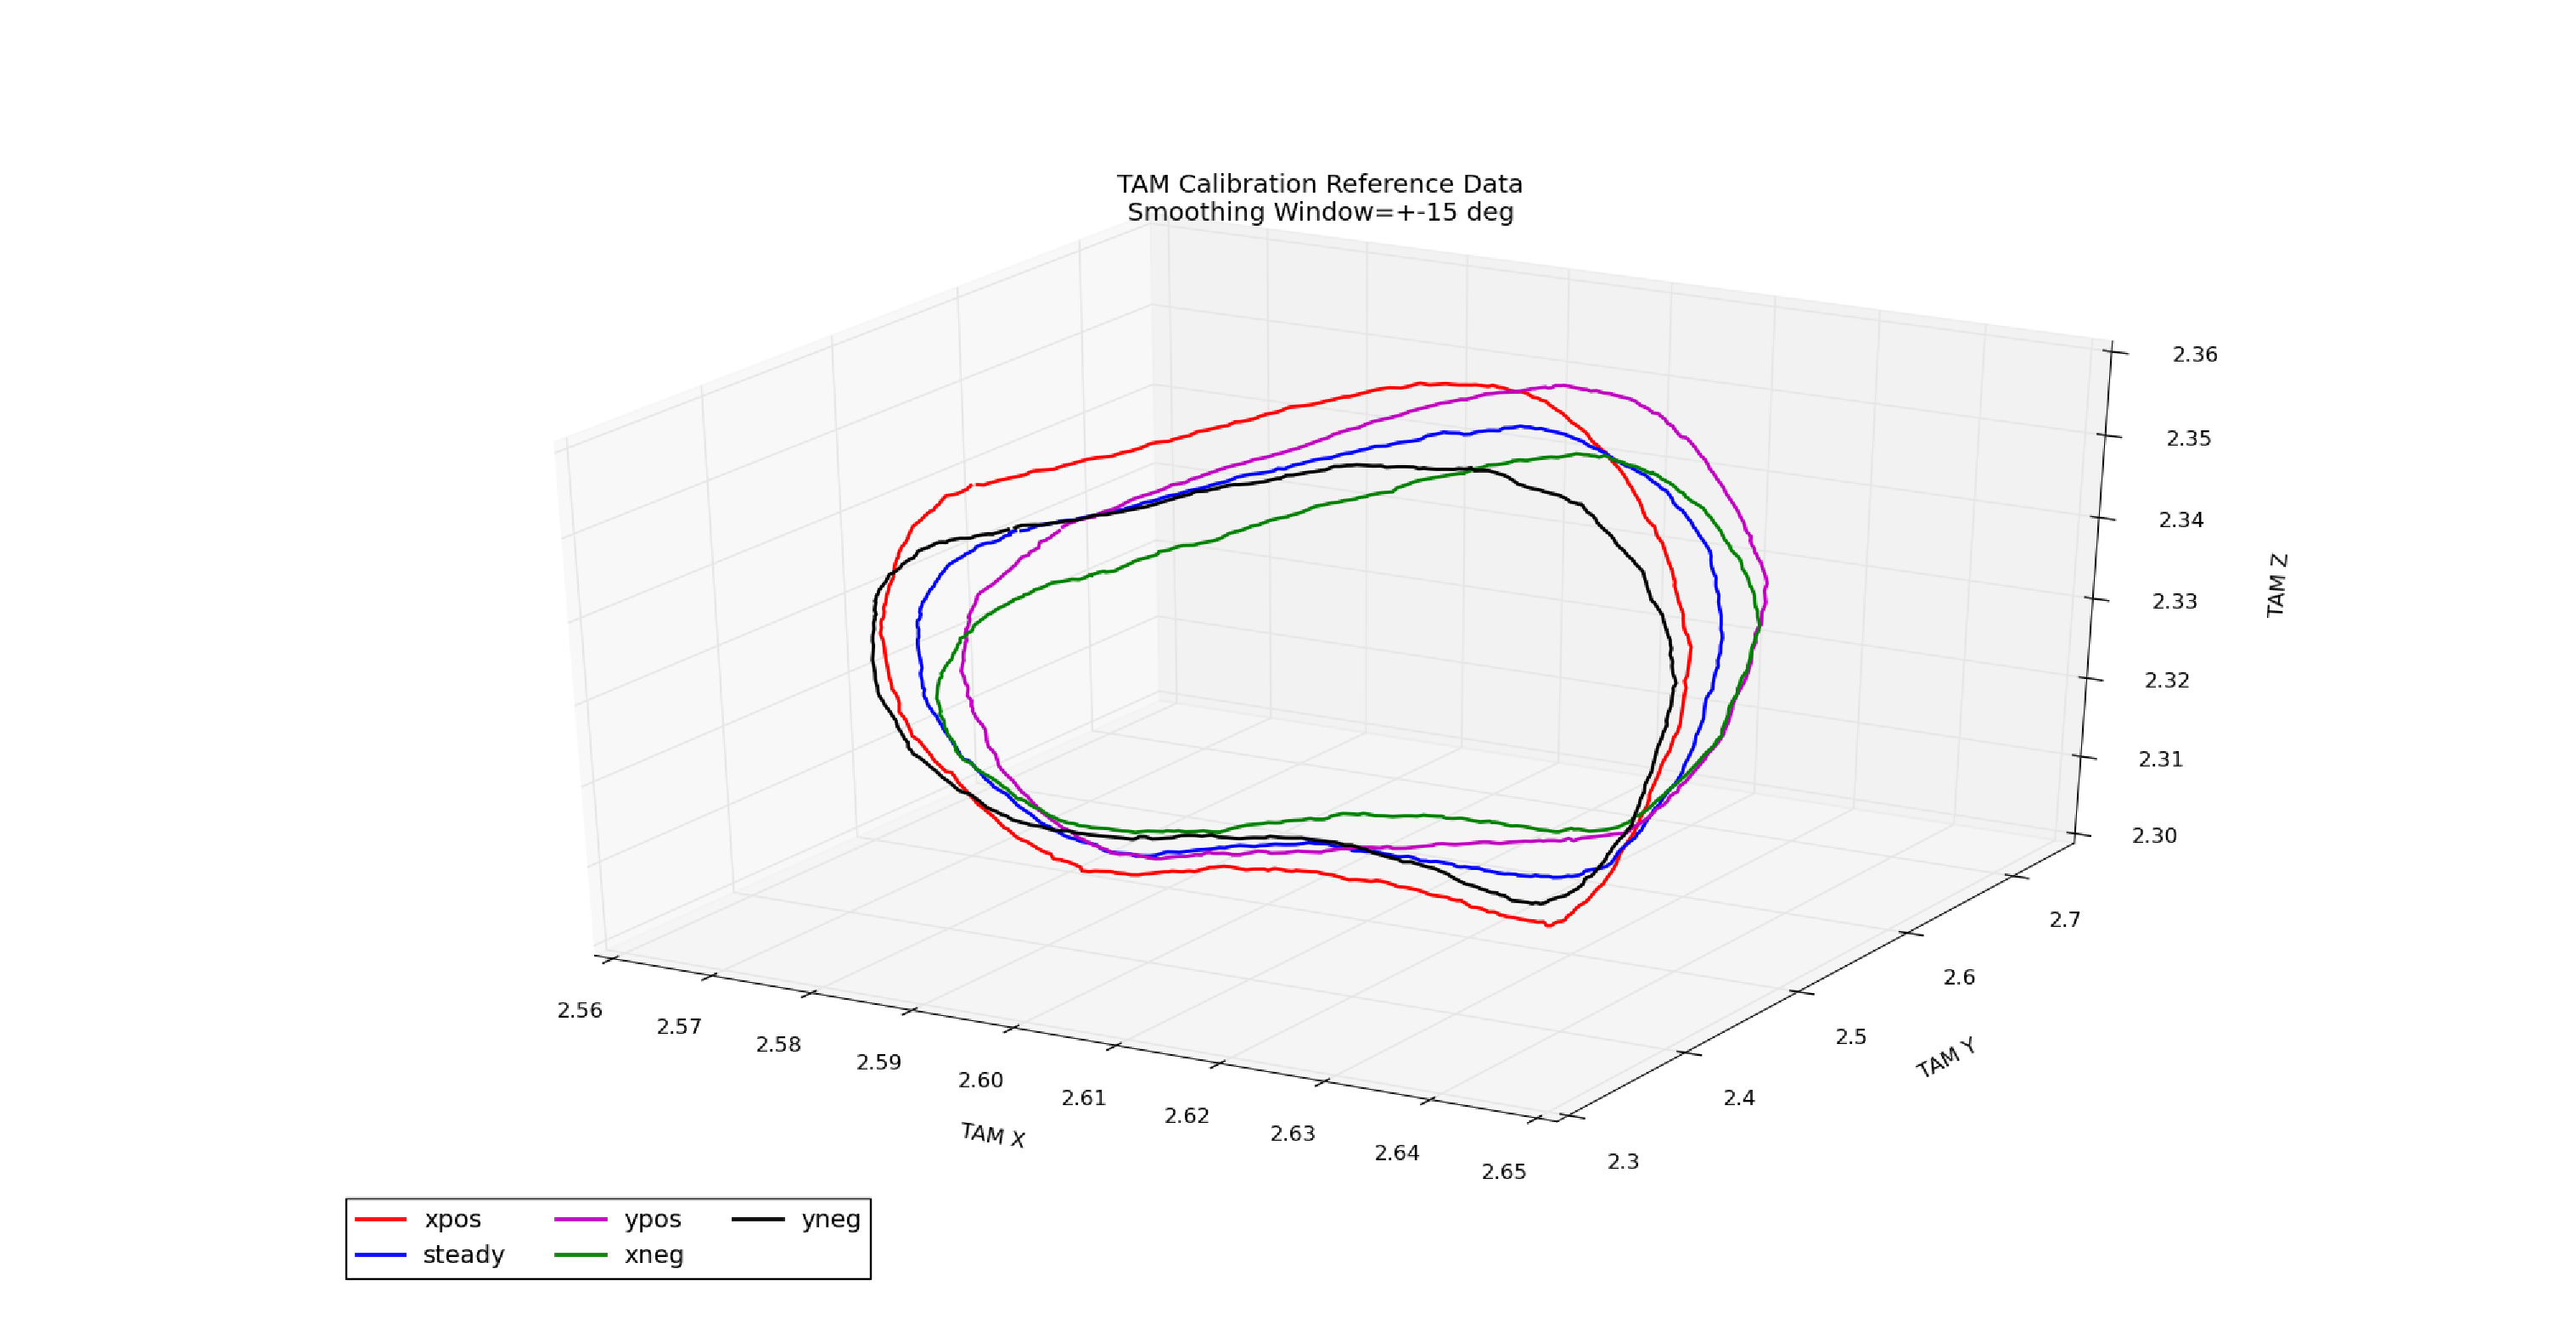
\includegraphics[width=\textwidth]{figures/tam_calibration_ref_15deg_smoothing.eps}
    \caption{$\pm 15^o$ smoothing}
    \label{fig:TAM15degCalibration}
  \end{subfigure}
  \caption{TAM Nutation Reference Values}
  \label{fig:TAMNutationReference}
\end{figure}

The cross shown in Figure \ref{fig:TAMRef191} illustrates the difference in the four nutation reference points compared to the stable point for a 191 degree yaw.  Figure \ref{fig:TAMPoints191} shows the level of noise reduction by the calibration process as the original data points are plotted against the reference nutation voltages.

\begin{figure}[H]
  \centerline{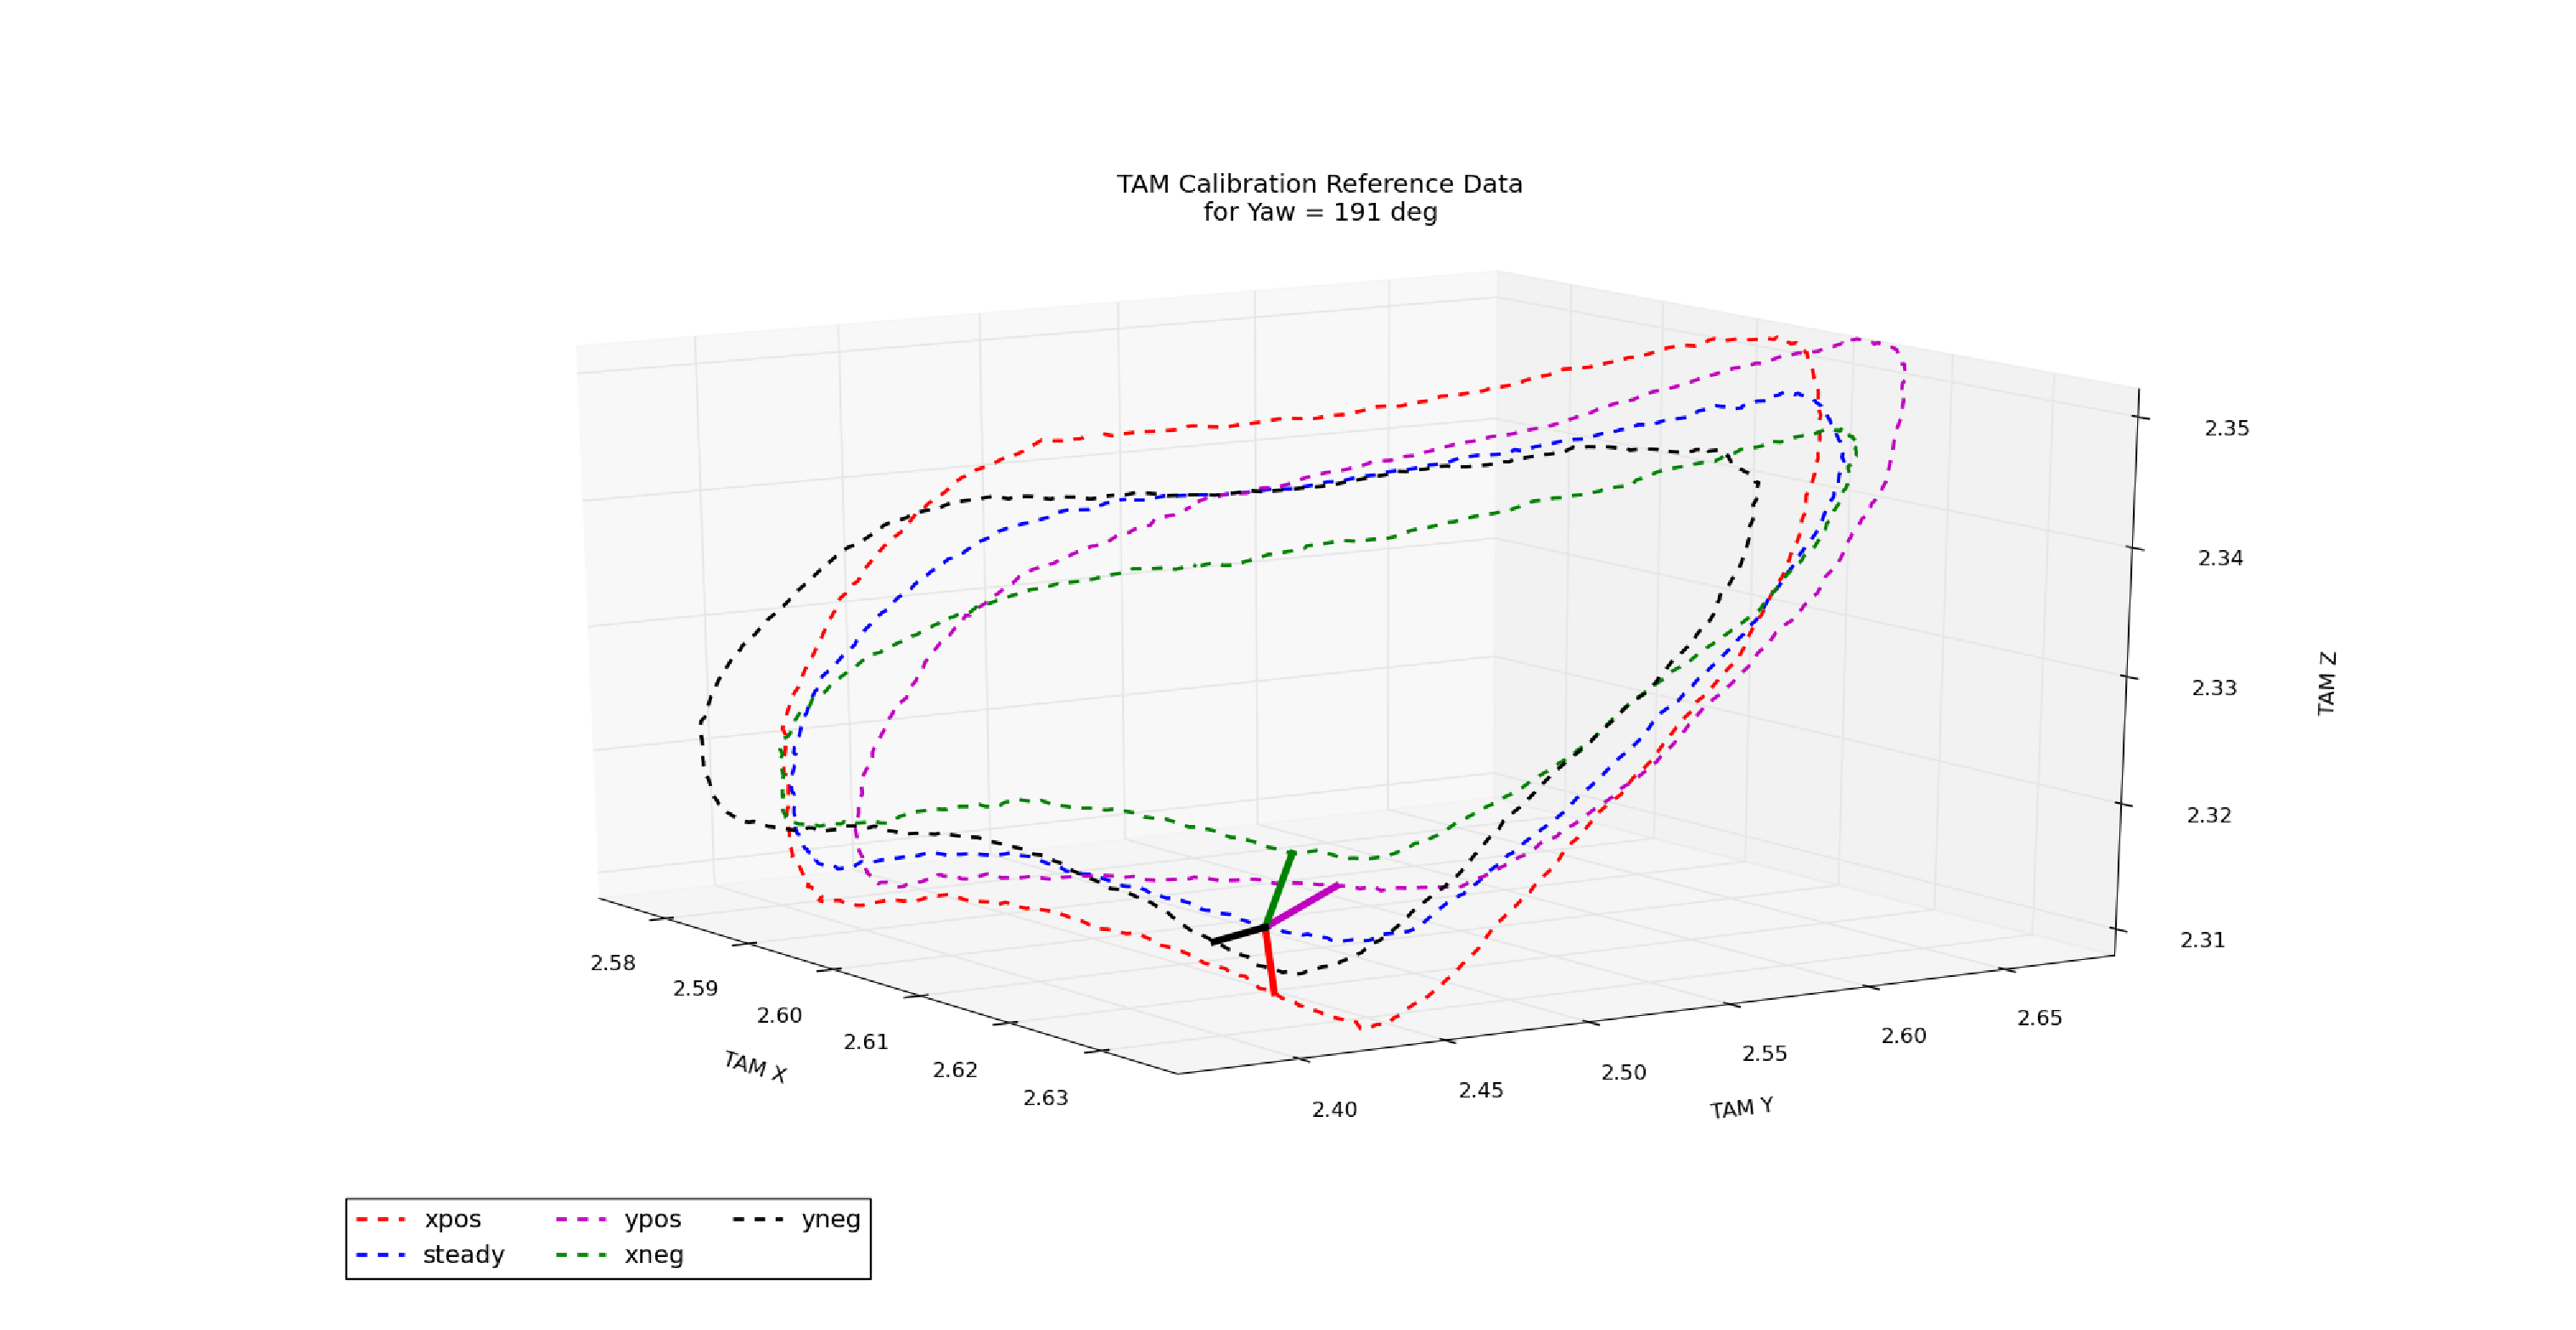
\psfig{file=figures/tam_calibration_ref_for_yaw_191.eps,height=3in}}
  \caption{TAM reference voltages for 191 degree yaw}
  \label{fig:TAMRef191}
\end{figure}

\begin{figure}[H]
  \centerline{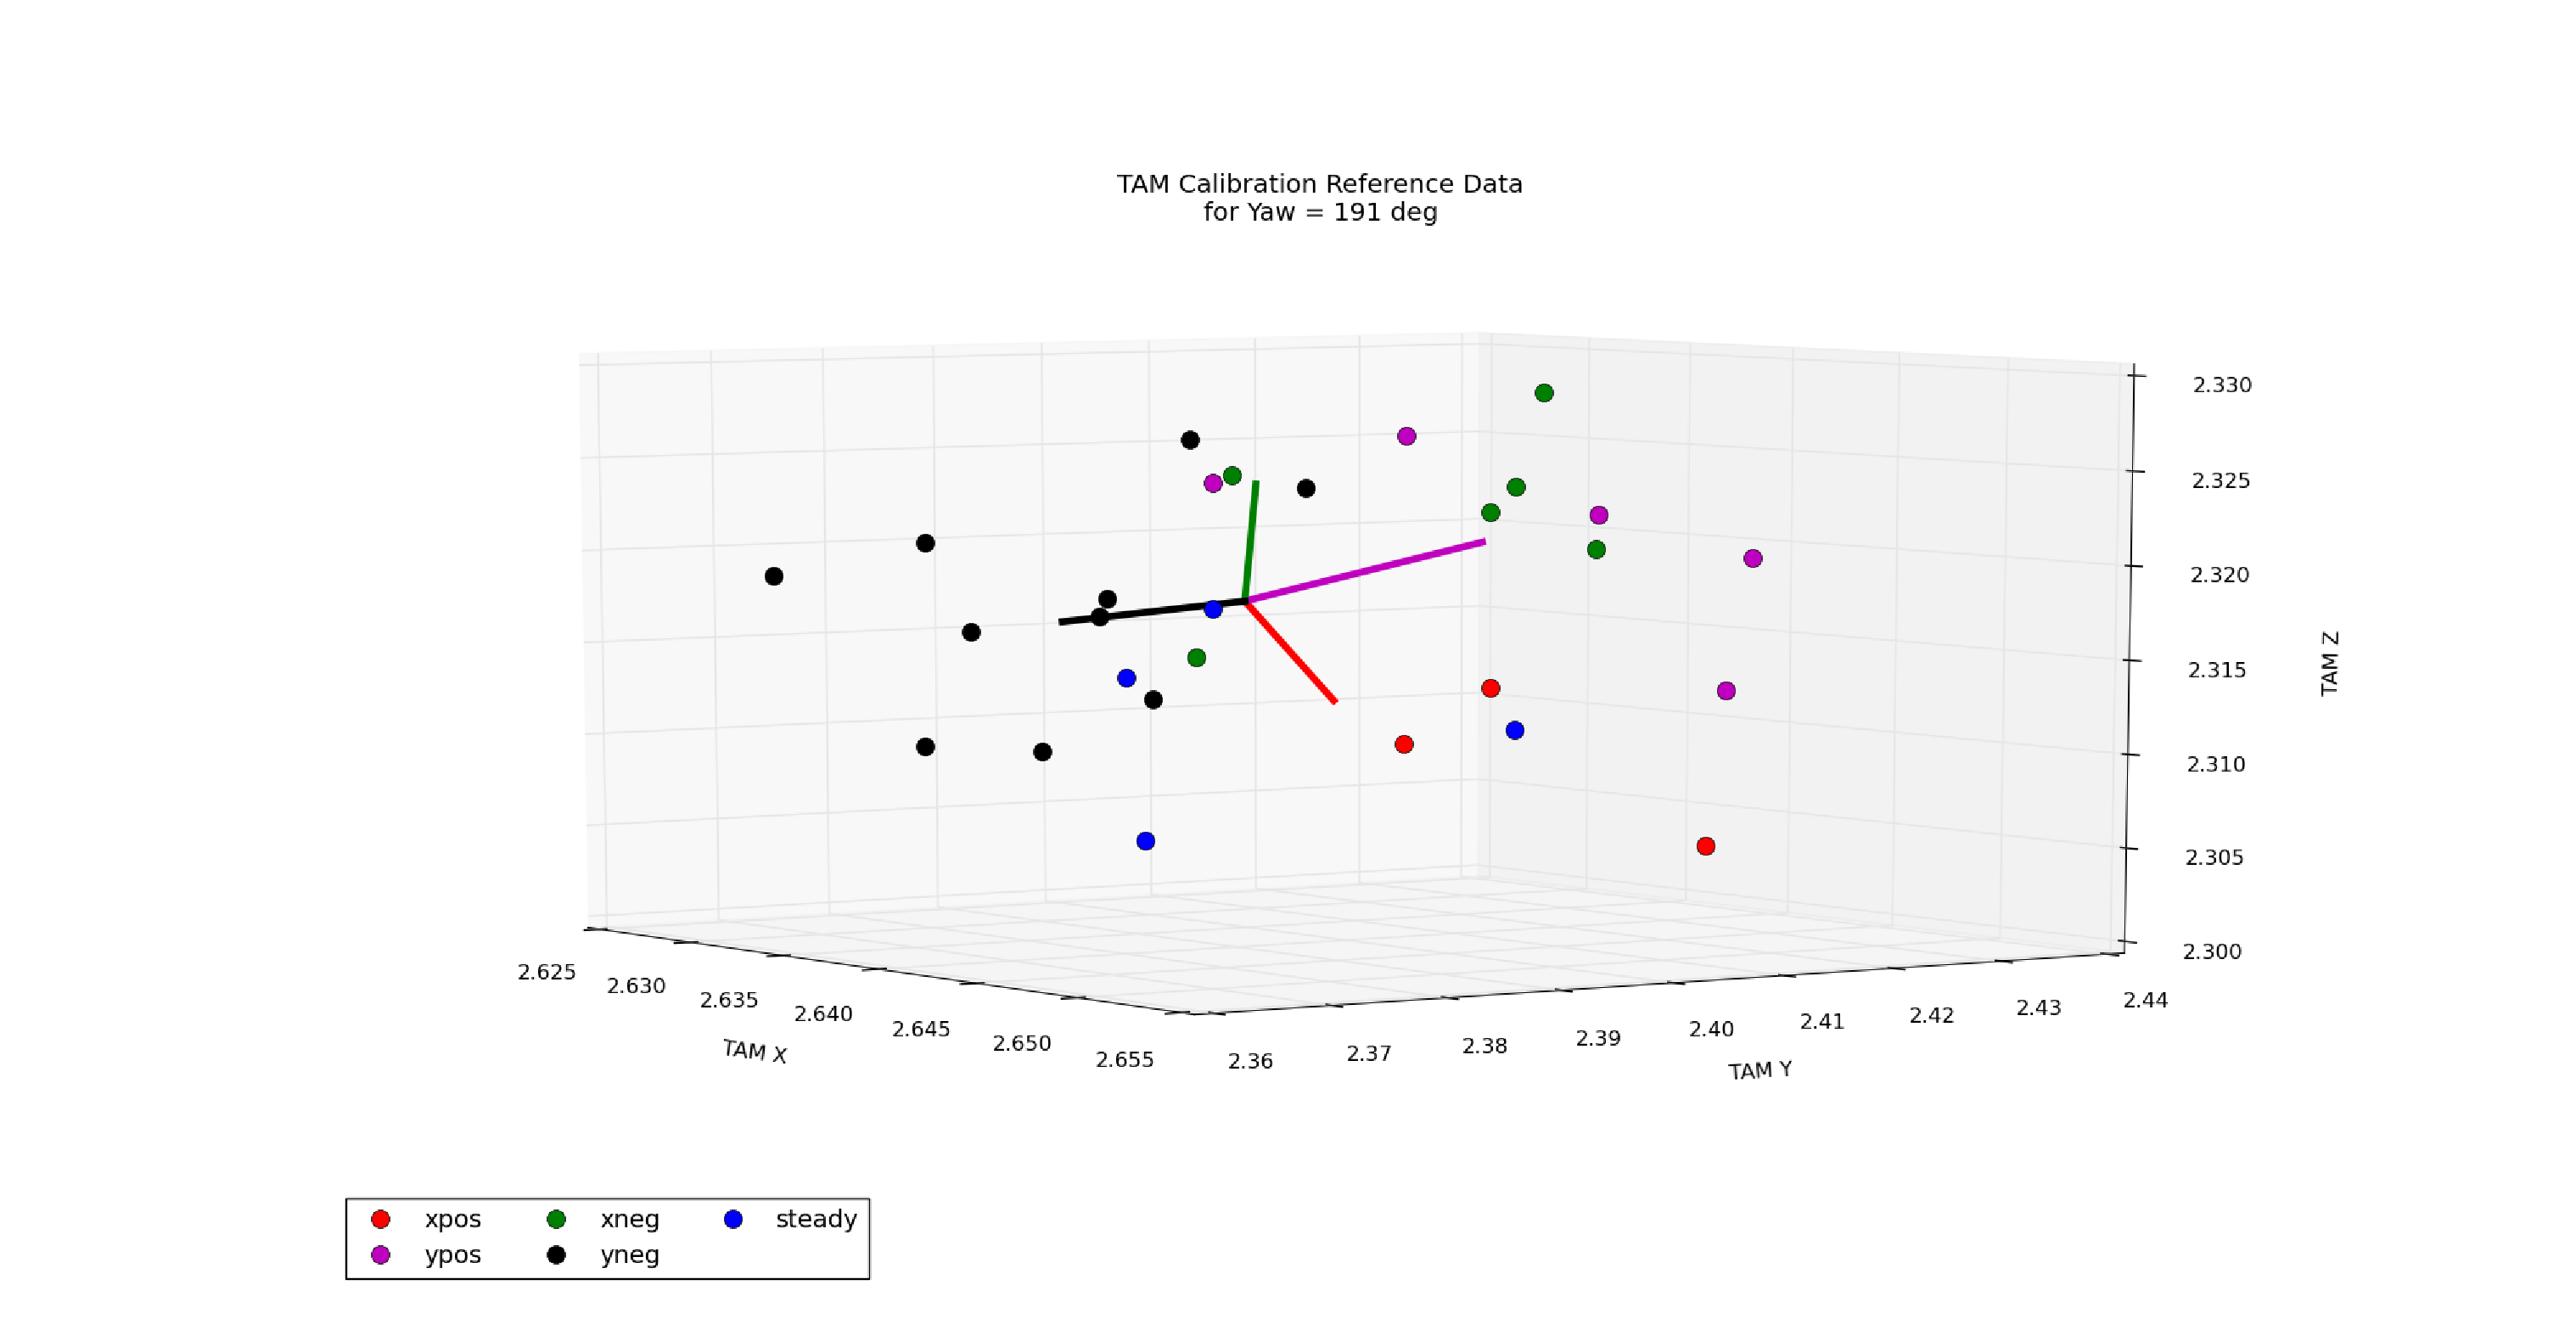
\psfig{file=figures/tam_calibration_191_degree_pts.eps,height=3in}}
  \caption{Closer view of TAM reference voltages for 191 degree yaw}
  \label{fig:TAMPoints191}
\end{figure}

\subsection{Estimating Nutation}

Taking one of the points from $-y$ calibration data to complete the example, Table \ref{tbl:TAMSamplePoints} lists the test point, along with the reference values, obtained from the calibration algorithm above.  The test point plotted in Figure \ref{fig:TAMPoint191} is nearest to the reference $-y$ value, but there is a large gap between the measured value and its associated reference, and other test points as in \ref{fig:TAMPoints191} are far closer to another reference point than its own.

\begin{table}[H]
  \centering
  \begin{tabular}{lc}
    \hline
    Test Point       & $(2.63, 2.37, 2.32)$ \\ \hline
    Steady Reference & $(2.63, 2.40, 2.32)$ \\ \hline
    xpos Reference   & $(2.63, 2.42, 2.31)$ \\ \hline
    ypos Reference   & $(2.64, 2.42, 2.32)$ \\ \hline
    xneg Reference   & $(2.64, 2.39, 2.32)$ \\ \hline
    yneg Reference   & $(2.63, 2.39, 2.32)$ \\ \hline
  \end{tabular}
  \caption{TAM sample reference points}
  \label{tbl:TAMSamplePoints}
\end{table}


\begin{figure}[H]
  \centerline{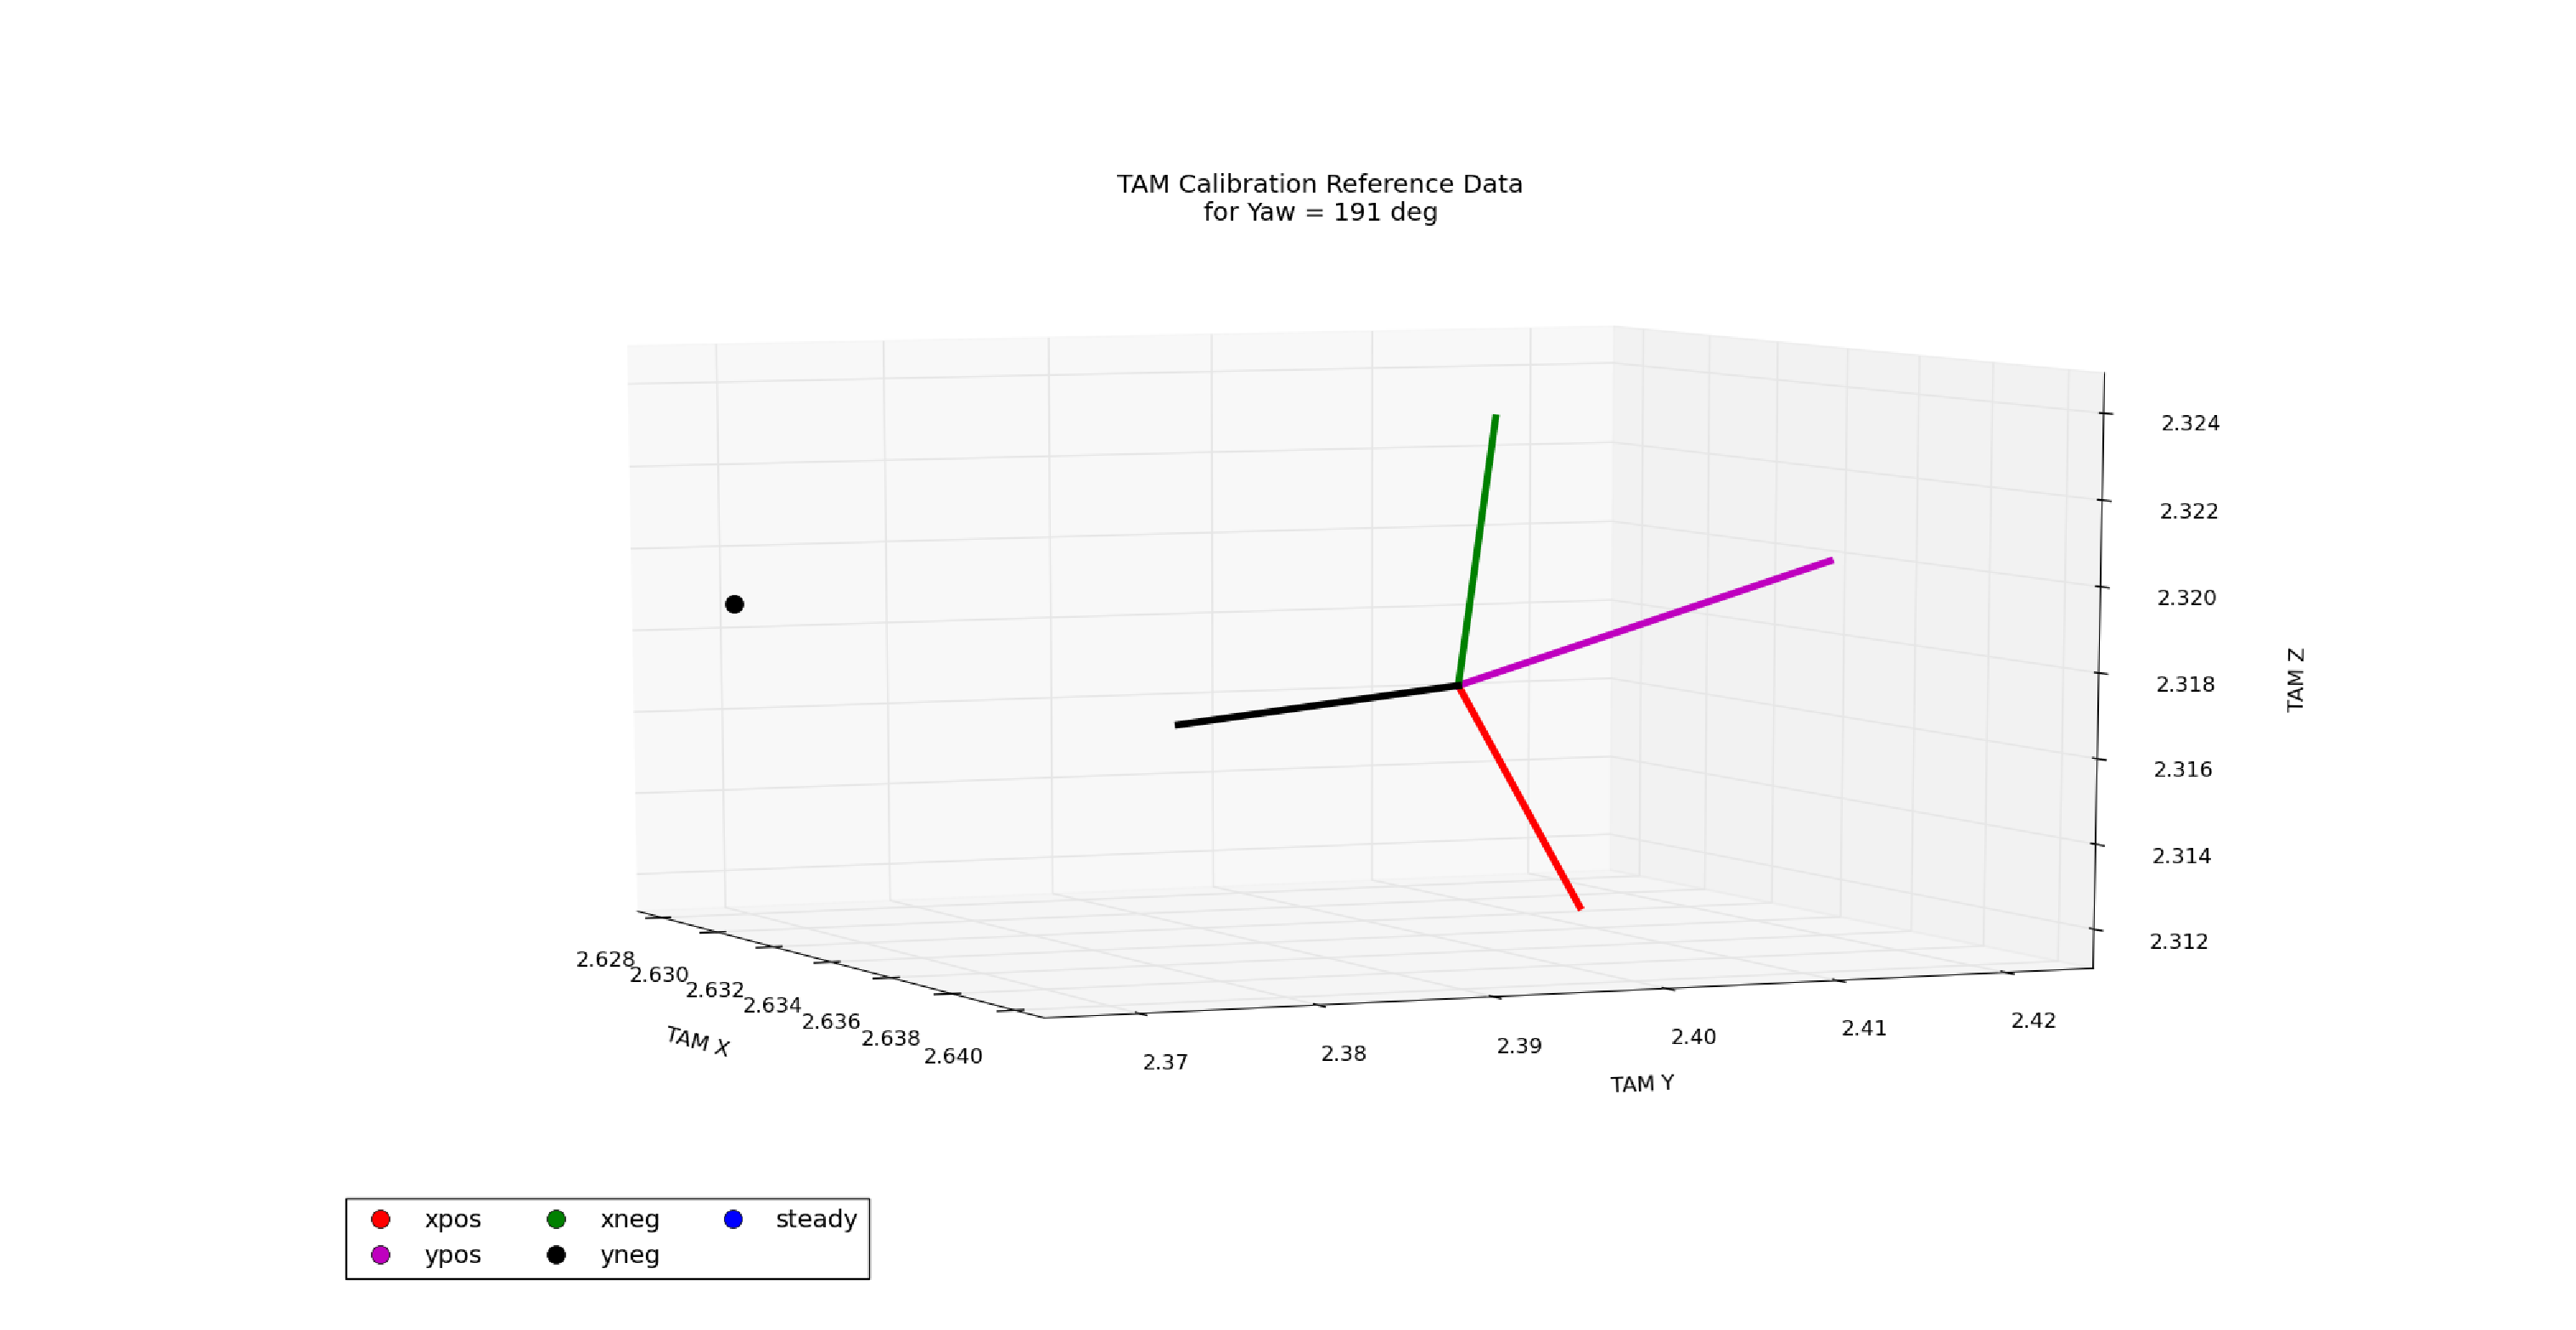
\psfig{file=figures/tam_calibration_191_degree_pt.eps,height=3in}}
  \caption{TAM sample data point for nutation calculation}
  \label{fig:TAMPoint191}
\end{figure}

In order to determine the best approximation for the measured nutations, a number of combinations of approaches are attempted including using the proportion between two estimates, normalizing the reference vectors, projecting the point to the plane consisting of the two nearest vectors, and creating a conversion of the x and y vectors to an orthogonal space.  Some cases provided slightly lower classification error rates when compared to the original calibration test set, but any improvements are not significant.  For simplicity and speed, the measurement estimate for nutation is reduced to a ``nearest neighbor'' classification \cite{nearestneighbor} where the closest reference point is chosen as the best approximation.

Despite the improved speed and simplicity, this classification method has some large faults, the biggest of which is the resulting chattered signal that is relayed to the estimator state.  This is because there are no continuum of values, the nutation state jumps between the five calibration states of level, and each of the $14^o$ nutations.  Further work is needed to refine this technique.
